\documentclass{article}
\usepackage[T1]{fontenc}
\usepackage[utf8]{inputenc}
\usepackage{amsmath}
\usepackage{tikz}
\usepackage{tikzsymbols}
\usepackage{lmodern}
\usetikzlibrary{arrows,automata}
\setlength\parindent{0pt}

\begin{document}

\begin{center}
  \Large{Informatik D - \"Ubungsblatt 2}

  \large{Sebastian H\"offner, Andrea Suckro}
\end{center}

\section{Aufgabe 2.1}

\textbf{Grammatik:}

\small
S $\rightarrow$ 0 | 1 | 2 | 3 | 4 | 5 | 6 | 7 | 8 | 9 | 1A | 2A | 3A | 4A | 5A | 6A | 7A | 8A | 9A \\
A $\rightarrow$ 0 | 1 | 2 | 3 | 4 | 5 | 6 | 7 | 8 | 9 | 0A | 1A | 2A | 3A | 4A | 5A | 6A | 7A | 8A | 9A

\normalsize
\textbf{Regul\"arer Ausdruck:}

(0|[1-9][0-9]*)

\section{Aufgabe 2.2}
\textbf{(a) } .*[\^{}a]\$

\textbf{(b) } .*00.*


\section{Aufgabe 2.3}
\textbf{(a) }

\textbf{Regul\"arer Ausdruck:} \Smiley\Smiley{[}\Smiley\Neutrey\Sadey{]}*\Sadey\Sadey

\textbf{Automat:}

\begin{center}
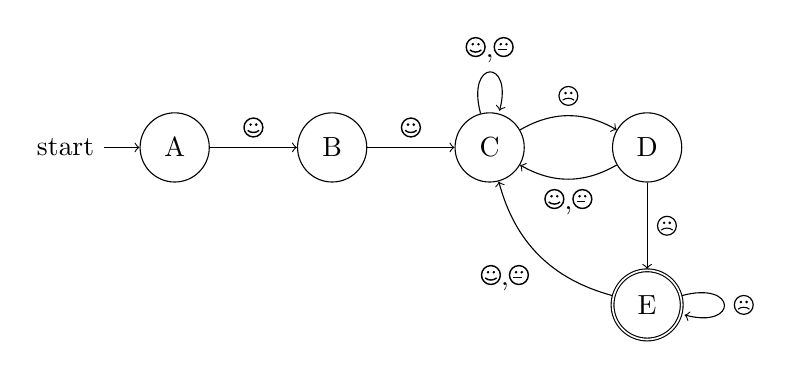
\begin{tikzpicture}[->,auto, node distance=2cm]
  \node[initial,state]   (A)              {A};
  \node[state]           (B) [right of=A] {B};
  \node[state]           (C) [right of=B] {C};
  \node[state]           (D) [right of=C] {D};
  \node[state,accepting] (E) [below of=D] {E};

  \path (A) edge              node {\Smiley}                 (B)
        (B) edge              node {\Smiley}                 (C)
        (C) edge [loop above] node {\Smiley,\Neutrey}        (C)
            edge [bend left]  node {\Sadey}                  (D)
        (D) edge              node {\Sadey}                  (E)
            edge [bend left]  node {\Smiley,\Neutrey}        (C)
        (E) edge [bend left]  node {\Smiley,\Neutrey}        (C)
            edge [loop right] node {\Sadey}                  (E)
        ;
\end{tikzpicture}
\end{center}

\newpage
\textbf{(b) }

\textbf{Regul\"arer Ausdruck:} ({[}\Smiley\Neutrey\Sadey{]}*\Neutrey\Neutrey)\{3\}{[}\Smiley\Neutrey\Sadey{]}*

\textbf{Automat:}

\begin{center}
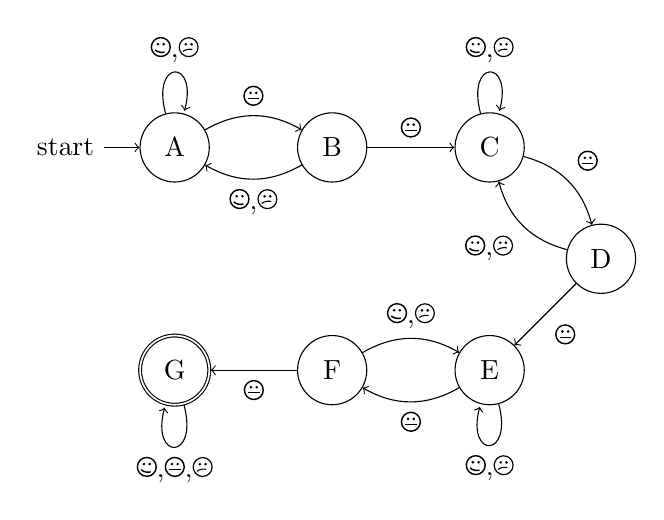
\begin{tikzpicture}[->,auto, node distance=2cm]
  \node[initial,state]   (A)                    {A};
  \node[state]           (B) [right of=A]       {B};
  \node[state]           (C) [right of=B]       {C};
  \node[state]           (D) [below right of=C] {D};
  \node[state]           (E) [below left of=D]  {E};
  \node[state]           (F) [left of=E]        {F};
  \node[state,accepting] (G) [left of=F]        {G};

  \path (A) edge [loop above] node {\Smiley,\Sadey}          (A)
            edge [bend left]  node {\Neutrey}                (B)
        (B) edge [bend left]  node {\Smiley,\Sadey}          (A)
            edge              node {\Neutrey}                (C)
        (C) edge [loop above] node {\Smiley,\Sadey}          (C)
            edge [bend left]  node {\Neutrey}                (D)
        (D) edge [bend left]  node {\Smiley,\Sadey}          (C)
            edge              node {\Neutrey}                (E)
        (E) edge [loop below] node {\Smiley,\Sadey}          (E)
            edge [bend left]  node {\Neutrey}                (F)
        (F) edge [bend left]  node {\Smiley,\Sadey}          (E)
            edge              node {\Neutrey}                (G)
        (G) edge [loop below] node {\Smiley,\Neutrey,\Sadey} (G)
        ;
\end{tikzpicture}
\end{center}

\textbf{(c) }

\textbf{Regul\"arer Ausdruck:} 

\small
({[}\Neutrey\Sadey{]}|\Smiley{[}\Neutrey\Sadey{]})*\Smiley\Smiley{[}\Neutrey\Sadey{]}({[}\Neutrey\Sadey{]}|\Smiley{[}\Neutrey\Sadey{]})*\Smiley\Smiley({[}\Neutrey\Sadey{]}(({[}\Neutrey\Sadey{]}|\Smiley{[}\Neutrey\Sadey{]})*|\Smiley))*

Alternativ:

({[}\Neutrey\Sadey{]}|\Smiley{[}\Neutrey\Sadey{]})*\Smiley\Smiley{[}\Neutrey\Sadey{]}({[}\Neutrey\Sadey{]}|\Smiley{[}\Neutrey\Sadey{]})*\Smiley\Smiley(({[}\Neutrey\Sadey{]}({[}\Neutrey\Sadey{]}|\Smiley{[}\Neutrey\Sadey{]})*)*|{[}\Neutrey\Sadey{]}\Smiley)
    
%( {[}\Neutrey\Sadey{]} | \Smiley {[}\Neutrey\Sadey{]} )*
%\Smiley\Smiley {[}\Neutrey\Sadey{]}
%( {[}\Neutrey\Sadey{]} | \Smiley {[}\Neutrey\Sadey{]} )*
%\Smiley\Smiley
    %( {[}\Neutrey\Sadey{]} 
        %( 
           %( {[}\Neutrey\Sadey{]} | \Smiley {[}\Neutrey\Sadey{]} )* | \Smiley
        %)
    %)*

\textbf{Automat:}

\begin{center}
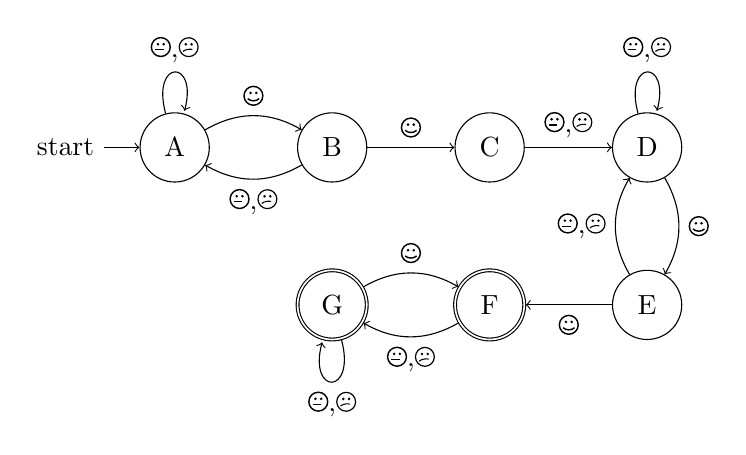
\begin{tikzpicture}[->,auto, node distance=2cm]
  \node[initial,state]   (A)              {A};
  \node[state]           (B) [right of=A] {B};
  \node[state]           (C) [right of=B] {C};
  \node[state]           (D) [right of=C] {D};
  \node[state]           (E) [below of=D] {E};
  \node[state,accepting] (F) [left of=E]  {F};
  \node[state,accepting] (G) [left of=F]  {G};

  \path (A) edge [loop above] node {\Neutrey,\Sadey} (A)
            edge [bend left]  node {\Smiley}         (B)
        (B) edge [bend left]  node {\Neutrey,\Sadey} (A)
            edge              node {\Smiley}         (C)
        (C) edge              node {\Neutrey,\Sadey} (D)
        (D) edge [loop above] node {\Neutrey,\Sadey} (D)
            edge [bend left]  node {\Smiley}         (E)
        (E) edge [bend left]  node {\Neutrey,\Sadey} (D)
            edge              node {\Smiley}         (F)
        (F) edge [bend left]  node {\Neutrey,\Sadey} (G)
        (G) edge [loop below] node {\Neutrey,\Sadey} (G)
            edge [bend left]  node {\Smiley}         (F)
        ;
\end{tikzpicture}
\end{center}

\newpage
\section{Aufgabe 2.4}

\textbf{Minimal gültiger Automat}

\begin{center}
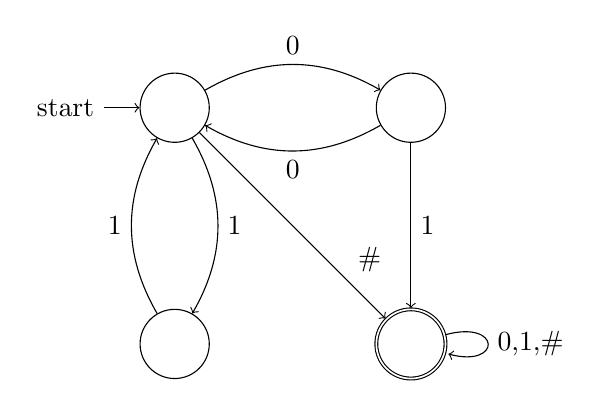
\begin{tikzpicture}[->,auto, node distance=3cm]
  \node[initial,state]   (A)              {};
  \node[state]           (B) [below of=A] {};
  \node[state]           (C) [right of=A] {};
  \node[state,accepting] (D) [below of=C] {};

  \path (A) edge [bend left]  node {1}      (B)
            edge [bend left]  node {0}      (C)
            edge [pos=0.8]    node {\#}     (D)
        (B) edge [bend left]  node {1}      (A)
        (C) edge [bend left]  node {0}      (A)
            edge              node {1}      (D)
        (D) edge [loop right] node {0,1,\#} (D)
        ;
\end{tikzpicture}
\end{center}

%\textbf{Garantiert gerade Anzahl Stellen}
%
%\begin{center}
%\begin{tikzpicture}[->,auto, node distance=2cm]
  %\node[initial,state,accepting](A)              {A};
  %\node[state]                  (B) [below of=A] {B};
  %\node[state]                  (C) [right of=A] {C};
  %\node[state,accepting]        (D) [right of=C] {D};
  %\node[state]                  (E) [right of=D] {E};
%
  %\path (A) edge [bend left] node {1}   (B)
            %edge [bend left] node {0}   (C)
        %(B) edge [bend left] node {1}   (A)
        %(C) edge [bend left] node {0}   (A)
            %edge             node {1}   (D)
        %(D) edge [bend left] node {0,1} (E)
        %(E) edge [bend left] node {0,1} (D)
        %;
%\end{tikzpicture}
%\end{center}

\textbf{Garantiert \#-terminiert}

\begin{center}
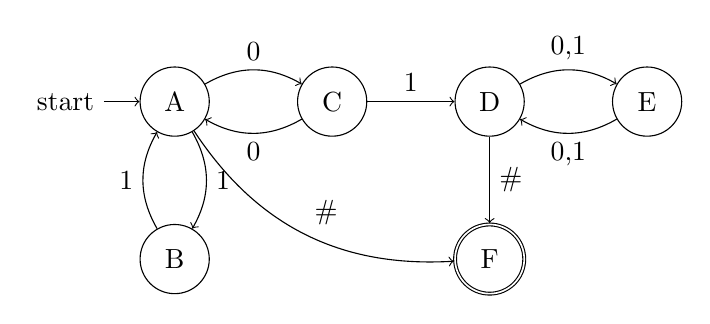
\begin{tikzpicture}[->,auto, node distance=2cm]
  \node[initial,state]   (A)              {A};
  \node[state]           (B) [below of=A] {B};
  \node[state]           (C) [right of=A] {C};
  \node[state]           (D) [right of=C] {D};
  \node[state]           (E) [right of=D] {E};
  \node[state,accepting] (F) [below of=D] {F};

  \path (A) edge [bend left]  node {1}   (B)
            edge [bend left]  node {0}   (C)
            edge [bend right] node {\#}  (F)
        (B) edge [bend left]  node {1}   (A)
        (C) edge [bend left]  node {0}   (A)
            edge              node {1}   (D)
        (D) edge [bend left]  node {0,1} (E)
            edge              node {\#}  (F)
        (E) edge [bend left]  node {0,1} (D)
        ;
\end{tikzpicture}
\end{center}

\textbf{Garantiert \#-terminiert und kein Akzeptieren des Leerworts}

\begin{center}
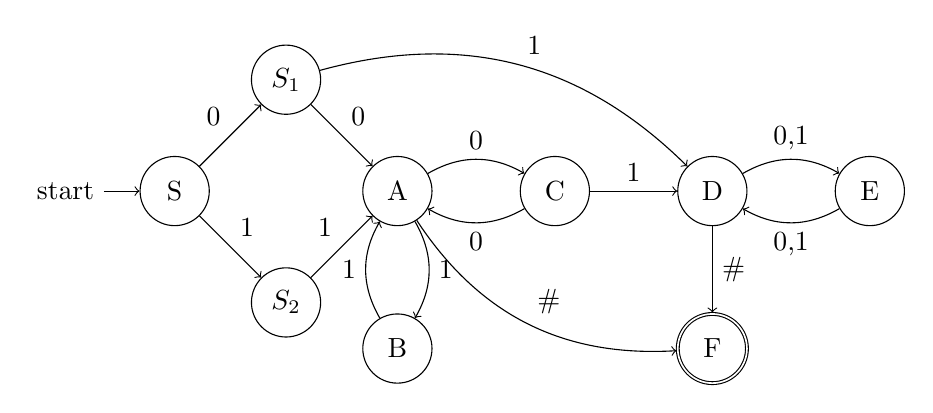
\begin{tikzpicture}[->,auto, node distance=2cm]
  \node[initial,state]   (S)              {S};
  \node[state]           (S1)[above right of=S]{$S_1$};
  \node[state]           (S2)[below right of=S]{$S_2$};
  \node[state]           (A) [below right of=S1]{A};
  \node[state]           (B) [below of=A] {B};
  \node[state]           (C) [right of=A] {C};
  \node[state]           (D) [right of=C] {D};
  \node[state]           (E) [right of=D] {E};
  \node[state,accepting] (F) [below of=D] {F};

  \path (S) edge              node {0}   (S1)
            edge              node {1}   (S2)
        (S1)edge              node {0}   (A)
            edge [bend left]  node {1}   (D)
        (S2)edge              node {1}   (A)
        (A) edge [bend left]  node {1}   (B)
            edge [bend left]  node {0}   (C)
            edge [bend right] node {\#}  (F)
        (B) edge [bend left]  node {1}   (A)
        (C) edge [bend left]  node {0}   (A)
            edge              node {1}   (D)
        (D) edge [bend left]  node {0,1} (E)
            edge              node {\#}  (F)
        (E) edge [bend left]  node {0,1} (D)
        ;
\end{tikzpicture}
\end{center}

\textbf{Andere Anordnung}

\begin{center}
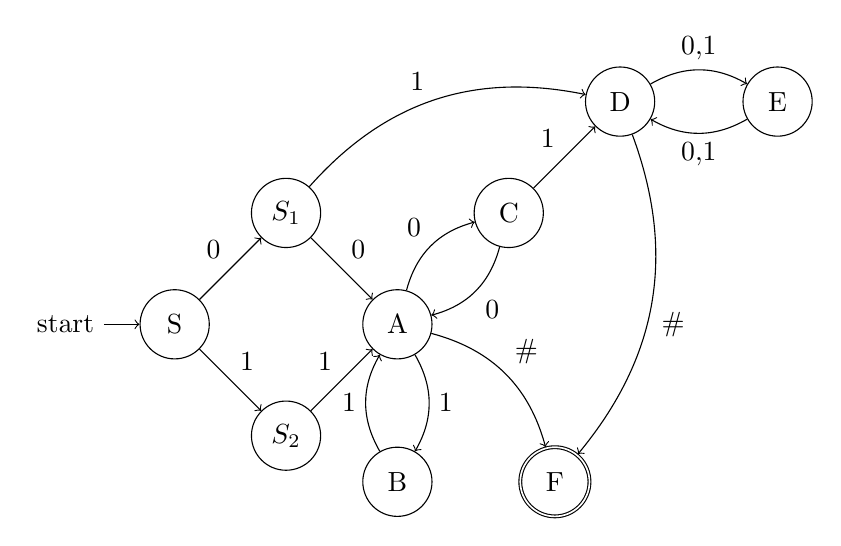
\begin{tikzpicture}[->,auto, node distance=2cm]
  \node[initial,state]   (S)              {S};
  \node[state]           (S1)[above right of=S]{$S_1$};
  \node[state]           (S2)[below right of=S]{$S_2$};
  \node[state]           (A) [below right of=S1]{A};
  \node[state]           (B) [below of=A] {B};
  \node[state]           (C) [above right of=A] {C};
  \node[state]           (D) [above right of=C] {D};
  \node[state]           (E) [right of=D] {E};
  \node[state,accepting] (F) [right of=B] {F};

  \path (S) edge              node {0}   (S1)
            edge              node {1}   (S2)
        (S1)edge              node {0}   (A)
            edge [bend left]  node {1}   (D)
        (S2)edge              node {1}   (A)
        (A) edge [bend left]  node {1}   (B)
            edge [bend left]  node {0}   (C)
            edge [bend left]  node {\#}  (F)
        (B) edge [bend left]  node {1}   (A)
        (C) edge [bend left]  node {0}   (A)
            edge              node {1}   (D)
        (D) edge [bend left]  node {0,1} (E)
            edge [bend left]  node {\#}  (F)
        (E) edge [bend left]  node {0,1} (D)
        ;
\end{tikzpicture}
\end{center}

\newpage
\section{Aufgabe 2.5}
\begin{figure}[h]
  \includegraphics[width=\textwidth]{crossword.png}
\end{figure}

\section{Aufgabe 2.6}
\begin{align*}
A &\rightarrow Ba\ |\ BCa\ |\ BCDa \\
B &\rightarrow a\  |\ bB\  |\ Ba\  |\ BB \\ %% BB bin ich noch nicht sicher, aber irgendwie muss aba produzierbar sein
C &\rightarrow a\  |\ aa\  |\ ada  \\
D &\rightarrow DD\ |\ c\   |\ cC   
\end{align*}

\end{document}